% !TeX program = xelatex
\documentclass{ctexart}
\usepackage{template_by_mny}
\usepackage{float} 
\usepackage{listings}

\title{量子密码学演示实验报告}
\class{物理 32/物理 31}
\name{冯家琦/周方远}
\id{2023011338/2023011263}

\begin{document}
\maketitle

\begin{abstract}
本实验通过EDU-QCRY1量子密码学演示套件,模拟和演示了量子密码学中的BB84协议原理。实验展示了量子密钥分发(QKD)的基本过程,包括密钥生成、消息加密传输以及窃听检测等关键环节。通过实验加深了对量子密码学原理的理解。
\end{abstract}

\section{实验原理}
\subsection{一次性密码本原理}
一次性密码本(One-Time Pad)是一种理论上完全安全的加密方法。它使用与明文等长的随机密钥,通过二进制加法对明文进行加密。加密过程需满足以下要求:
\begin{itemize}
\item 密钥长度不短于明文
\item 密钥只能使用一次
\item 密钥必须完全随机
\item 密钥只能由发送方和接收方知道
\end{itemize}

具体的加密算法为:Alice 将每位明文异或上对应位密钥作为密文,Bob 收到密文后将每位异或上对应位密钥即可得到明文。
\subsection{BB84协议}
BB84协议是一种量子密钥分发协议,用于安全地在通信双方间建立共享密钥。其基本步骤为:
\begin{enumerate}
\item 定义两组基底:+基(0°和90°偏振)和×基(-45°和45°偏振)
\item Alice随机选择基底发送随机比特
\item Bob随机选择基底进行测量
\item 通过公开信道交换使用的基底信息
\item 保留使用相同基底的测量结果作为密钥
\end{enumerate}

\section{实验仪器}
\begin{itemize}
\item 铝制光学平台
\item 635nm激光二极管模块
\item lambda/2波片
\item 偏振分束器
\item 光电探测器
\item 旋转支架
\item 控制电路
\item 其他光学支架和紧固件
\end{itemize}

\section{实验步骤}
\subsection{系统调试}
\begin{enumerate}
\item 安装激光器并调节光路
\item 校准lambda/2波片的角度设置
\item 调节探测器的灵敏度
\end{enumerate}

\begin{figure}[htbp]
    \centering
    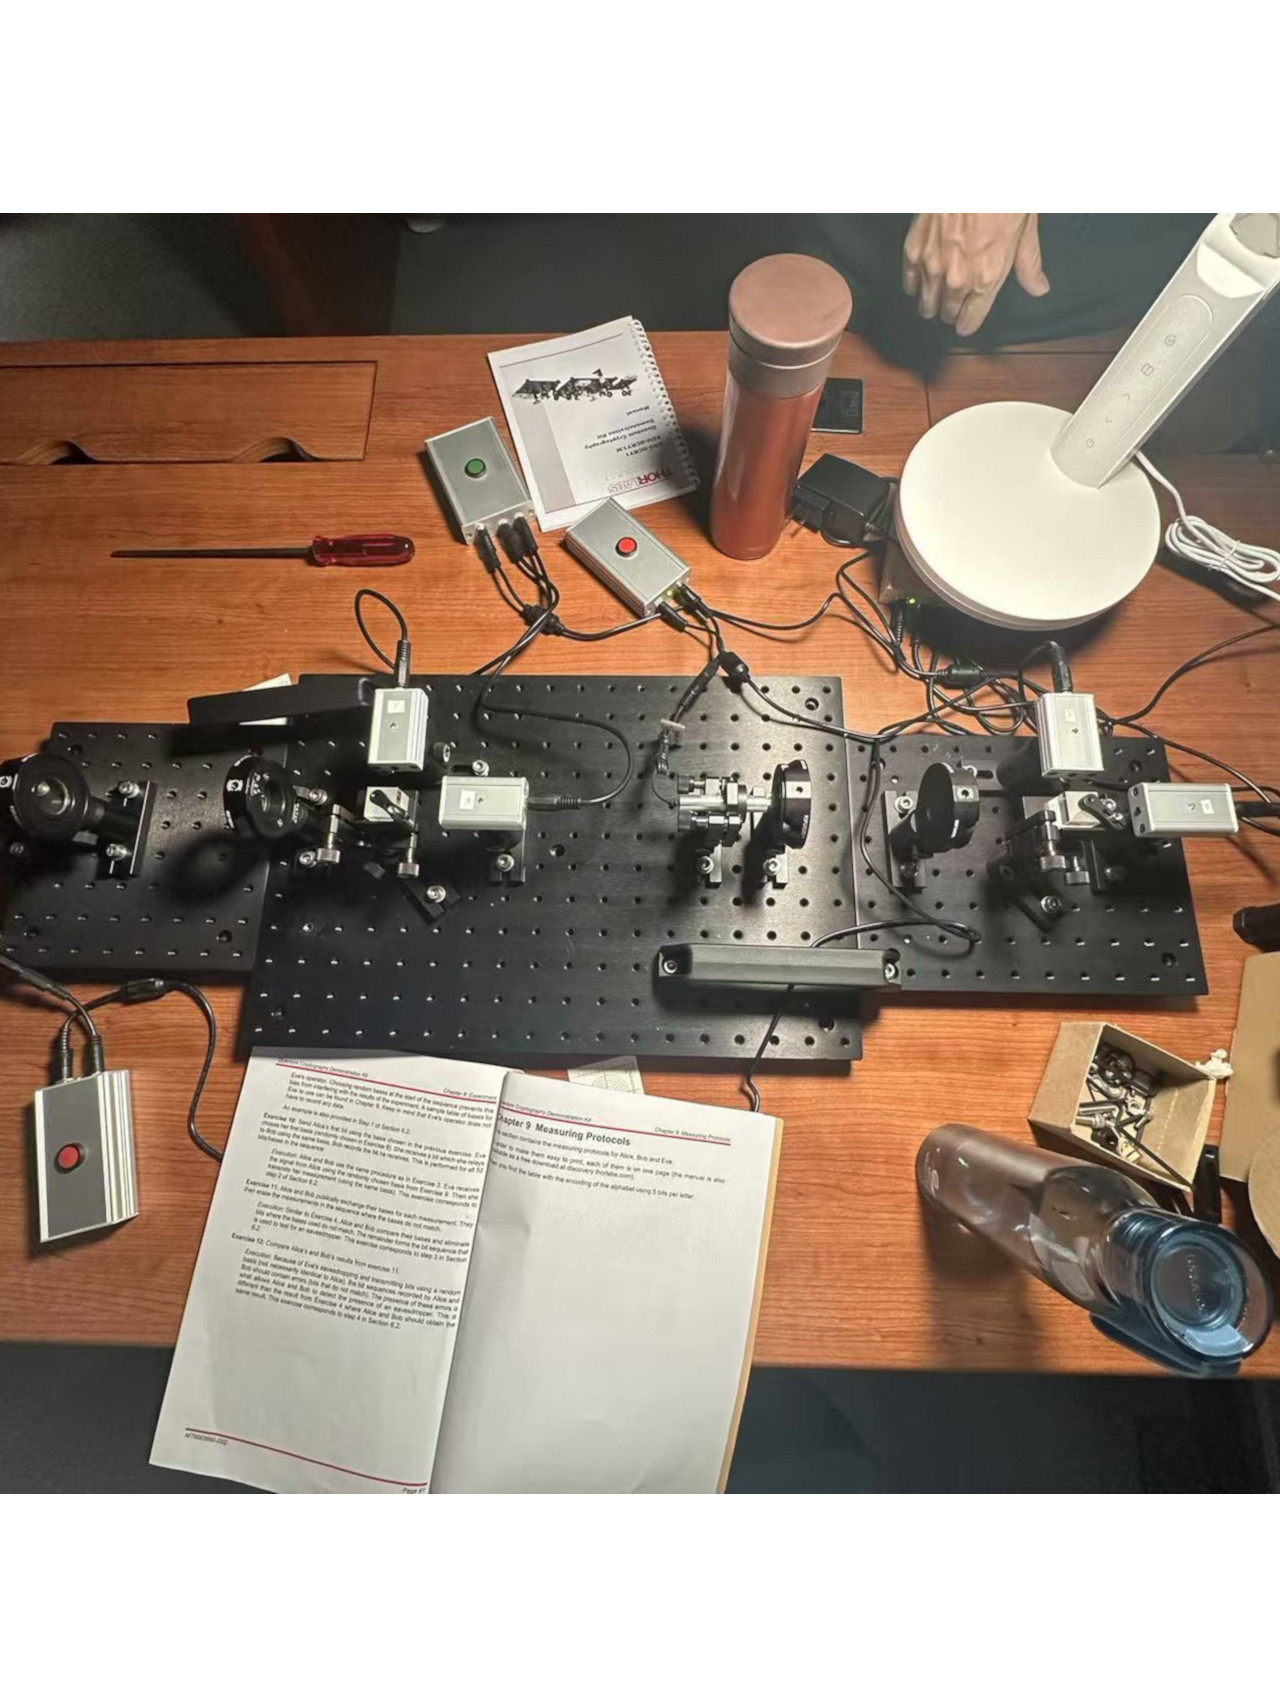
\includegraphics[width=0.2\textwidth,height=0.3\textwidth]{pictures/微信图片_20241031162855.jpg}
    \caption{包含 Bob, Eve, Alice 的完整实验系统}
\end{figure}

\subsection{密钥生成实验}
先将实验平台中的 Eve 部分移除,重新校对好 Alice 和 Bob,确保对于 Alice 发射的四种可能偏振与 Bob 测量偏振的两种可能基底的任意组合均能得到正确结果。

\begin{figure}[htbp]
    \centering
    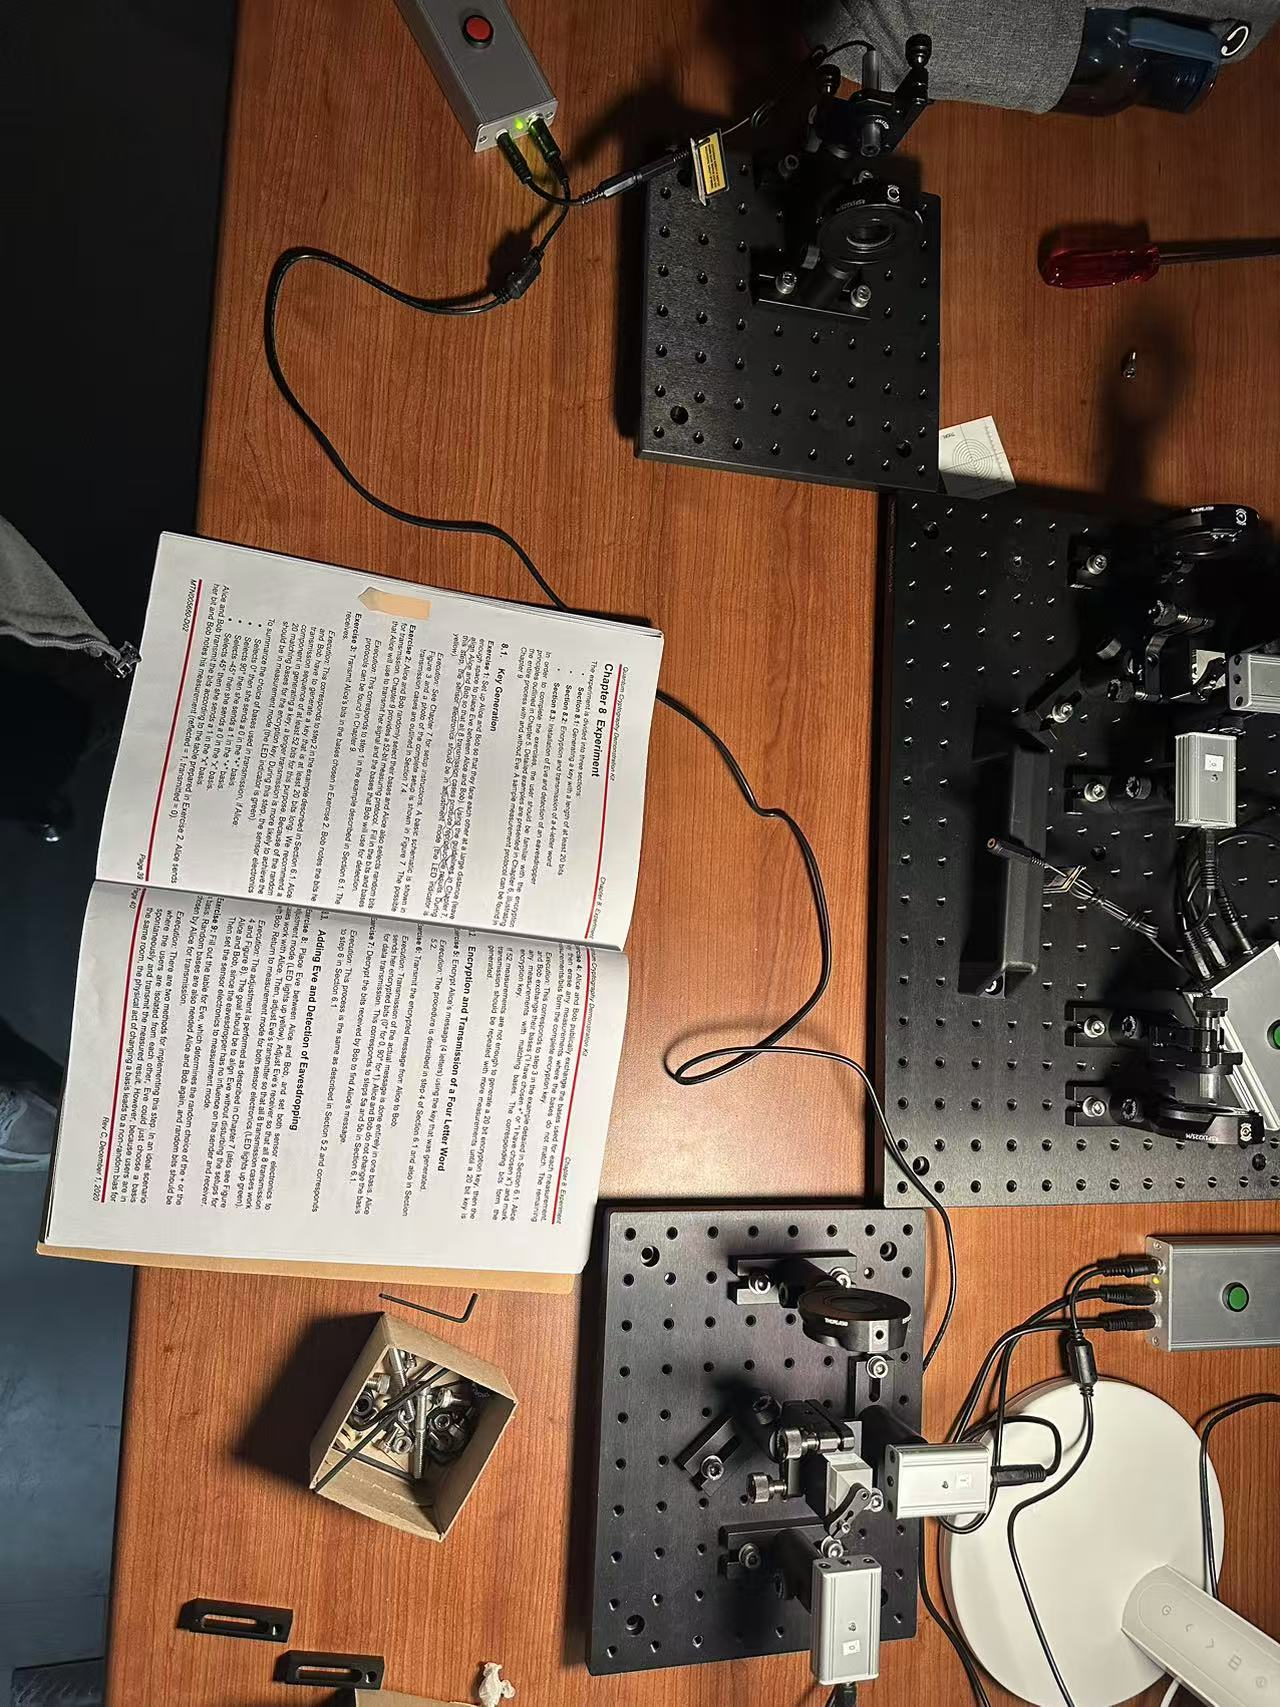
\includegraphics[width=0.2\textwidth,height=0.3\textwidth]{pictures/微信图片_20241031162758.jpg}
    \caption{仅包含 Bob, Alice 的实验系统}
\end{figure}

Alice 生成两段 52 bits 的随机基底和密钥,Bob 生成一段 52 bits 的随机基底。
    Alice Base: x+x++xxx+x++++xx+x+xxx+x++x++++++x+x+xxx+xx++xxx++xx
    Alice Key:  
    
    Bob Base:   xx++++x++x++x+++xx+x+x++++x++xxxx+xx++xx+x+x+++++x+x

Alice 用其选择的基底发送其生成的密钥,Bob 用自己选择的基底测量收到的光子。
\begin{enumerate}
\item 设置Alice和Bob的基底选择装置
\item 进行一系列比特传输
\item 记录双方使用的基底和测量结果
\item 通过比对确定共享密钥
\end{enumerate}

\subsection{窃听检测实验}
\begin{enumerate}
\item 在光路中加入Eve的测量装置
\item 重复密钥生成过程
\item 分析错误率变化
\end{enumerate}

\section{实验思考}
\begin{enumerate}
\item 本实验使用的是脉冲激光而非单光子源,这与实际的量子密码系统有何区别?
\item BB84协议中为什么要使用两组不同的基底?
\item 在有窃听者的情况下,为什么会出现约25\%的错误率?
\item 量子密码学相比经典密码学有哪些优势和局限性?
\end{enumerate}

\section{总结}
\begin{itemize}
\item 通过实验成功演示了BB84量子密钥分发协议的工作原理
\item 验证了窃听检测机制的有效性
\item 理解了量子密码学中的关键概念如基底选择、量子测量等
\item 掌握了量子通信系统的基本组成和调试方法
\end{itemize}

\end{document}